\documentclass[11pt]{standalone}
\usepackage{amssymb}
\usepackage{amsmath}
\usepackage[no-math]{fontspec}
\usepackage{unicode-math}
\setmainfont{Libertinus Sans}
\setsansfont{Libertinus Sans}
\setmathfont{Libertinus Math}
\usepackage{pgf,xcolor}
\usepackage{tikz}
\usetikzlibrary{arrows.meta, backgrounds}
\usepackage{pgfplots}
\pgfplotsset{compat=newest}

\definecolor{my_darkgray}{HTML}{484949}
\definecolor{my_lightgray}{HTML}{F3F4F4}
\definecolor{my_darkblue}{HTML}{005A94}
\definecolor{my_lightblue}{HTML}{CCDEE9}
\definecolor{my_yellow}{HTML}{FFEC7F}
\definecolor{my_red}{HTML}{E60000}
\definecolor{my_orange}{HTML}{E87846}

\begin{document}
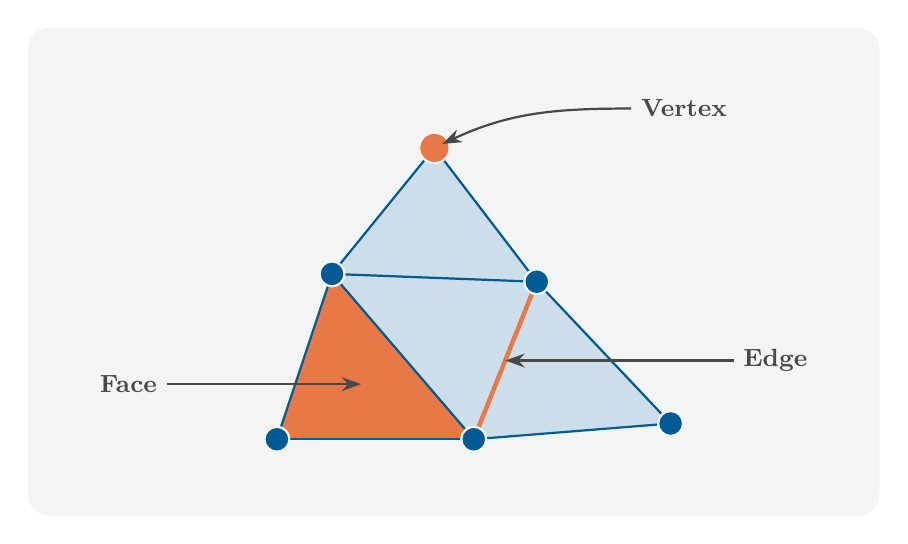
\begin{tikzpicture}[
    show background rectangle,
    background rectangle/.style={fill=my_lightgray, rounded corners=8pt},
    inner frame sep=0.8cm,
    annotation/.style={draw=my_darkgray, thick, -{Stealth[length=7pt, width=5pt]}}
]

% --- Vertex-Koordinaten ---
\coordinate (V1) at (0.0, 0.0);
\coordinate (V2) at (2.5, 0.0);
\coordinate (V3) at (5.0, 0.2);
\coordinate (V4) at (0.7, 2.1);
\coordinate (V5) at (3.3, 2.0);
\coordinate (V6) at (2.0, 3.7);

% --- Faces: Füllung (zuerst, damit Kanten darüber erscheinen) ---
% Hervorgehobene Face (my_orange)
\fill[my_orange]    (V1) -- (V2) -- (V4) -- cycle;
% Übrige Faces (my_lightblue)
\fill[my_lightblue] (V2) -- (V3) -- (V5) -- cycle;
\fill[my_lightblue] (V2) -- (V5) -- (V4) -- cycle;
\fill[my_lightblue] (V4) -- (V5) -- (V6) -- cycle;

% --- Edges: alle Kanten in my_darkblue ---
\draw[my_darkblue, thick] (V1) -- (V2);
\draw[my_darkblue, thick] (V2) -- (V3);
\draw[my_darkblue, thick] (V1) -- (V4);
\draw[my_darkblue, thick] (V2) -- (V4);
\draw[my_darkblue, thick] (V3) -- (V5);
\draw[my_darkblue, thick] (V4) -- (V5);
\draw[my_darkblue, thick] (V4) -- (V6);
\draw[my_darkblue, thick] (V5) -- (V6);

% Hervorgehobene Edge (my_orange, ultra thick)
\draw[my_orange, ultra thick] (V2) -- (V5);

% --- Vertices: Kreise mit weißem Ring ---
\foreach \v in {V1, V2, V3, V4, V5} {
    \fill[my_darkblue] (\v) circle (4.5pt);
    \draw[my_lightgray, thick] (\v) circle (4.5pt);
}

% Hervorgehobener Vertex (my_orange)
\fill[my_orange] (V6) circle (5.5pt);
\draw[my_lightgray, thick] (V6) circle (5.5pt);

% --- Annotationen ---
% Face: Schwerpunkt von V1-V2-V4 ≈ (1.07, 0.70)
\node[font=\small, text=my_darkgray, anchor=east] (lbl_face)
    at (-1.4, 0.7) {\textbf{Face}};
\draw[annotation] (lbl_face.east) -- (1.07, 0.70);

% Edge: Mittelpunkt von V2-V5 = (2.9, 1.0)
\node[font=\small, text=my_darkgray, anchor=west] (lbl_edge)
    at (5.8, 1.0) {\textbf{Edge}};
\draw[annotation] (lbl_edge.west) -- (2.9, 1.0);

% Vertex: V6 = (2.0, 3.7)
\node[font=\small, text=my_darkgray, anchor=west] (lbl_vertex)
    at (4.5, 4.2) {\textbf{Vertex}};
\draw[annotation] (lbl_vertex.west) to[out=180, in=25] (2.1, 3.75);

\end{tikzpicture}
\end{document}
